\section{Experiments}

The model has been tested in a series of benchmark environments, each with a different number of arms and reward distributions. The performance has been compared with the following algorithms: Random Baseline, Upper-Confidence Bound (UCB), Thompson Sampling, and Epsilon-Greedy.

% Description of the environments
\subsection{Game variants}\label{sec:envs}

% \noindent The game environments considered in this work are non-stationary K-Armed Bandits with Binomial rewards.
% In particular, the agent is evaluated over a number $T_{\text{trials}}$ of \textit{trials}, each composed by an arbitrary number $T_{\text{rounds}}$ of \textit{rounds}; each \textit{trial} is characterized by a different reward distribution $\mathbf{p}\sim\mathcal{U}(0,1)^{K}$ (although in practice the bounds have been set to $(0.1, 0.9)$ such that the distributions are less trivial).
\noindent Our goal is to investigate the performance of the agent in a non-stationary environment, meaning that its underlying distribution changes over time \footnote{Since the arm probabilities are not normalized to $1$, it is
technically improper to call them \textit{probability distributions}; we will therefore refer to either \textit{probability} or \textit{distribution} separately at any given time for avoiding confusion.}
We choose this setting as it resembles an ecological scenario in which an animal has to forage in an environment with food (reward) is distributed over a set of fixed locations, but whose occurrence probability can change over time.
Four different variants were used, obtained by introducing different types of non-stationarity: piecewise constant, uniformly changing, sinusoidally changing, and sinusoidally changing with piecewise constant arms.
The reason for these choices is to test the model performance under different speed and uniformity of the distribution changes.
Figure \ref{fig:envs} visually illustrates their specificities.

\hfill \break
\noindent \textbf{Piecewise stationary environment} [\textsc{KAB-P}]\\ Within a trial the reward distribution is stationary and it is drawn from a normal $\mathbf{p}=\mathcal{N}(0.5, 0.2)^{K}$, clipped in $(0, 1)$. At the end of each trial $i$ it is drawn a new distribution $\mathbf{\mathbf{p}}_{i} \to \mathbf{\mathbf{p}}_{i+1}$ \cite{qiForcedExplorationBandit2023}.

\hfill \break
\noindent \textbf{Piecewise stationary environment with drift} [\textsc{KAB-D}]\\ At the very beginning, the reward distribution $\mathbf{p}$ is sampled from a normal $\mathbf{p}=\mathcal{N}(0.5, 0.2)^{K}$.
Then, it changes gradually over the rounds, tracked as time $t$, such that its values tend towards a target distribution $\mathbf{q}_{i}$ as $\tau_{p}\dot{\mathbf{p}}_{t}=\mathbf{q}_{i}-\mathbf{p}_{t}$.
Here, $\dot{\mathbf{p}}$ is the time derivative of the distribution and $\tau_{p}$ is its time constant.
Once the distance is below a threshold $\delta$ as $\vert \mathbf{q}_{i} - \mathbf{p}_{t}\vert < \delta$, the target distribution is changed to a new one $\mathbf{q}_{i}\to\mathbf{q}_{i+1}$. In this variant, there are no proper trials but the target distribution keep changing until a maximum number
of rounds is reached.

\hfill \break
\noindent \textbf{Sinusoidal distribution shift} [\textsc{KAB-$\sin$}]\\ The reward distribution changes over rounds, with the probability of each arm following a sine wave with a specific frequency $f_{k}$, phase $\lambda_{k}$ and amplitude $1$. At any given time $t$, the distribution is $\mathbf{p}_{t}=\{\sin(2\pi f_{k} t+\lambda_{k})\text{  for }k=1\ldots K\}$.

\hfill \break
\noindent \textbf{Partial sinusoidal distribution shift} [\textsc{KAB-$\sin$P}]\\ Identical to the sinusoidal distribution shift, but only a subset of the arms changes sinusoidally while the rest is kept at a constant value and the distribution is not normalized.


\begin{figure}[ht]
    \centering
    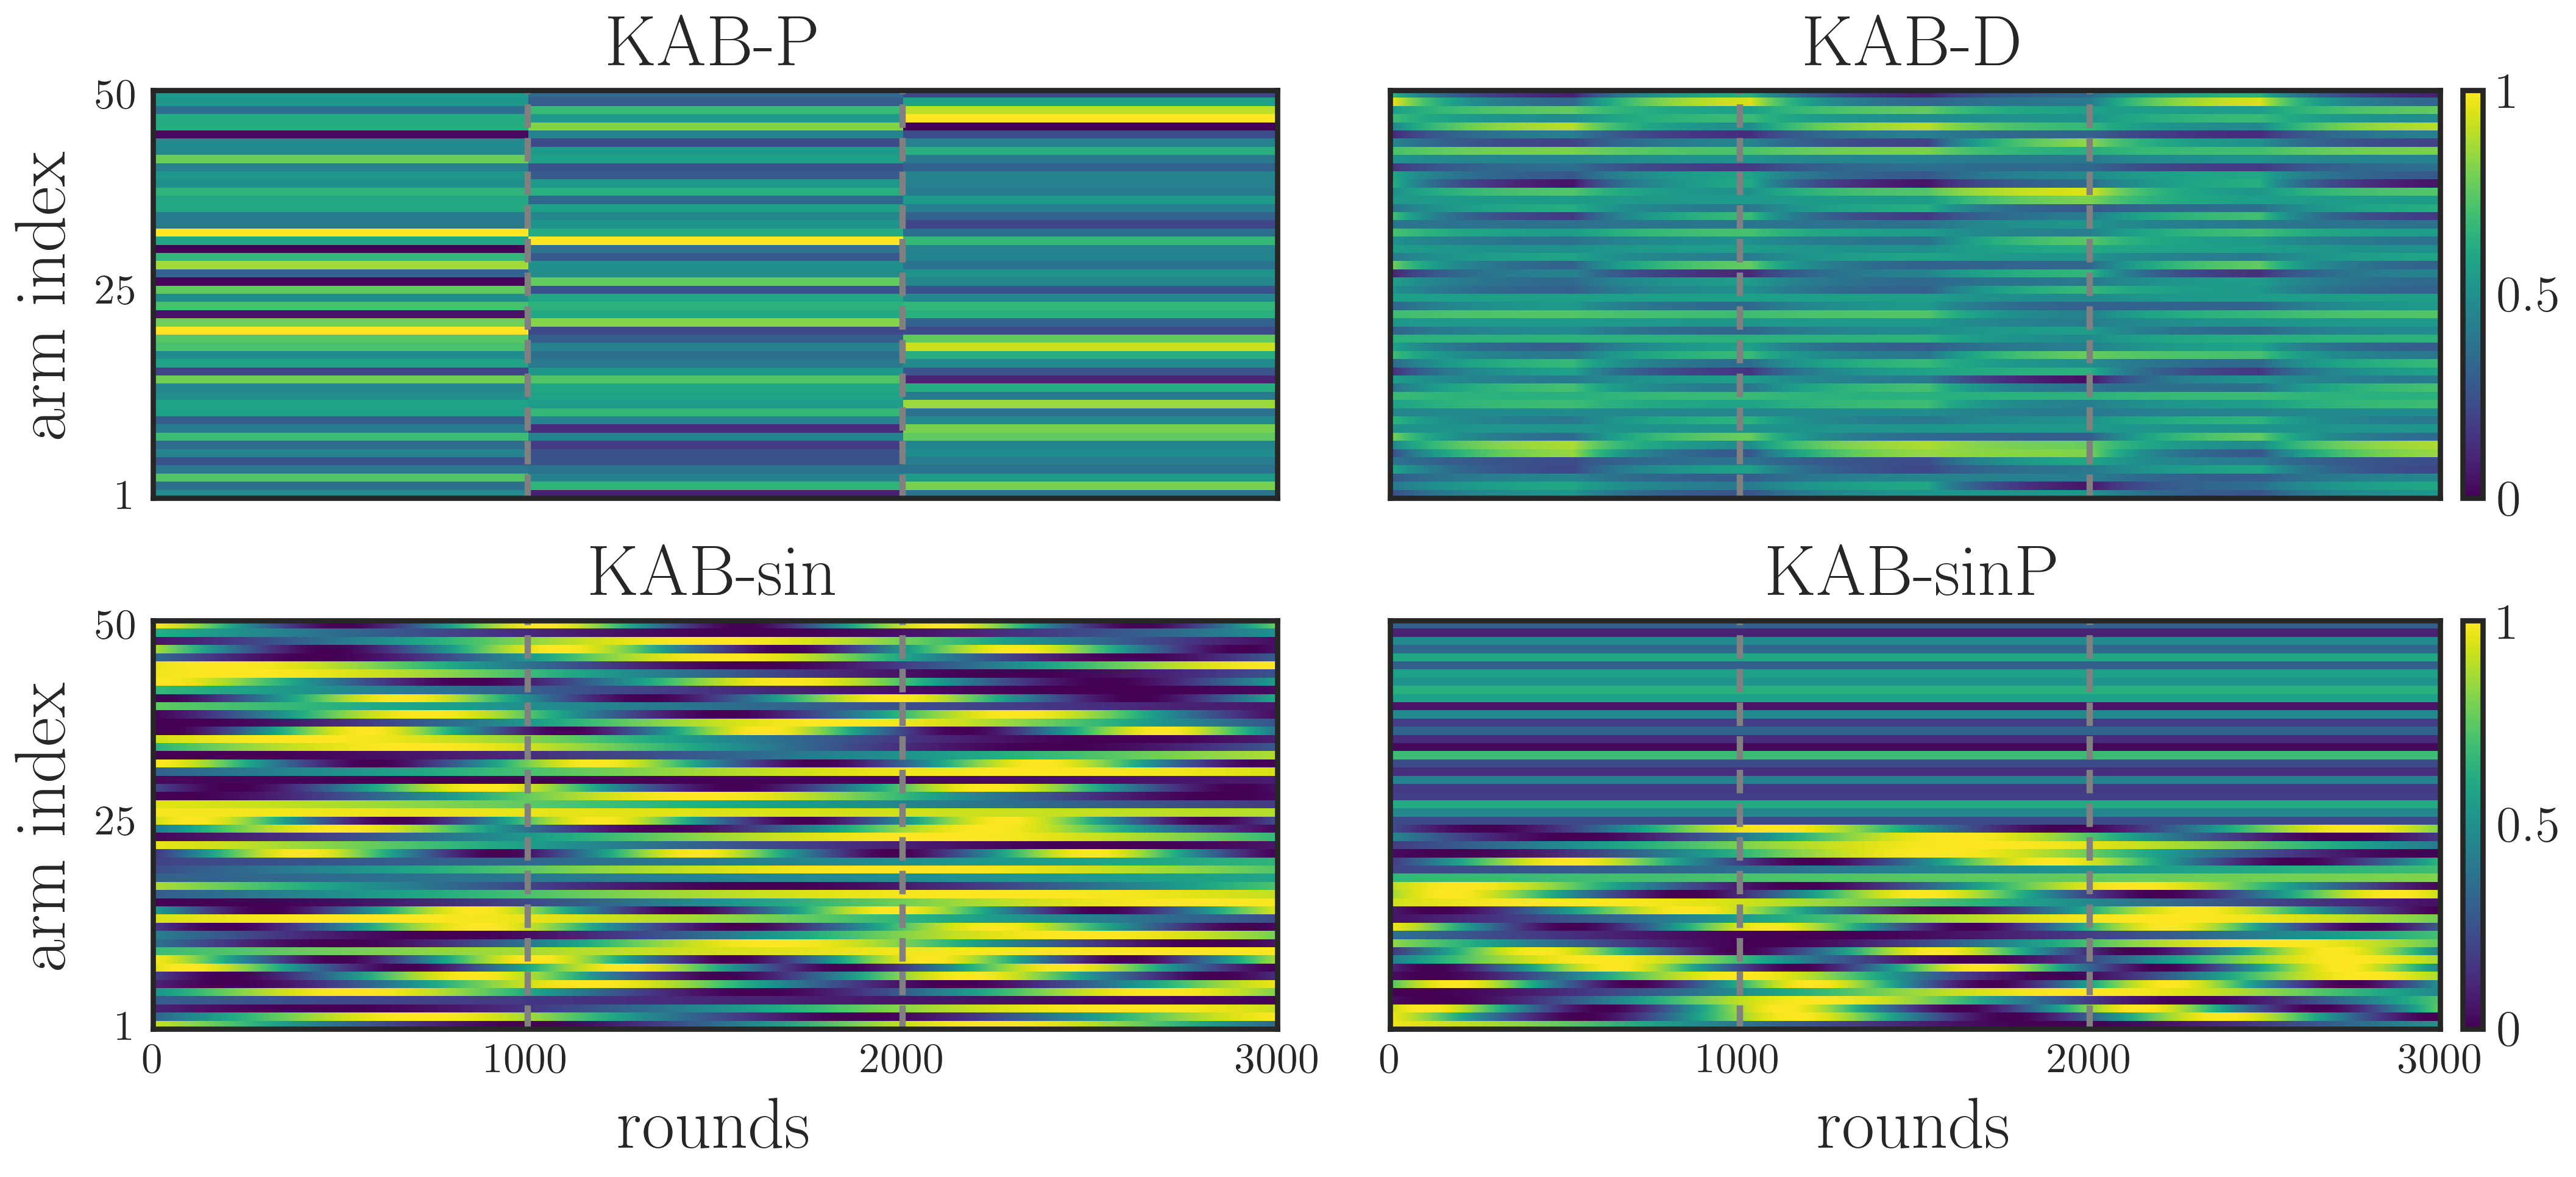
\includegraphics[width=1.\textwidth]{figures/envs_1.png}
    \caption{\textsc{Reward distribution for the four game variants} - \textit{The reward distribution for each arm and environment is plotted over three trials of 1000, demarcated by a dotted grey line.}}
    \label{fig:envs}
\end{figure}


% Evolution: fitness evolution
\subsection{Evolution search}
The optimization of the hyper-parameters was performed using the Covariance Matrix Adaptation evolutionary strategy algorithm (CMA-ES) \cite{igelCovarianceMatrixAdaptation2007}.
The search was run with a population of $256$ individuals for $80$ generations. Each individual was endowed with a genome, corresponding to a vector of 22 parameters of the model.
The fitness function of the evolution was defined as the average reward obtained by an individual over 3 different non-stationary bandit environments, each for $K=\{40, 200\}$, and all averaged over 2 iterations.
The results are summarized below in figure \ref{fig:evolution}.

\begin{figure}[H]
    \centering
    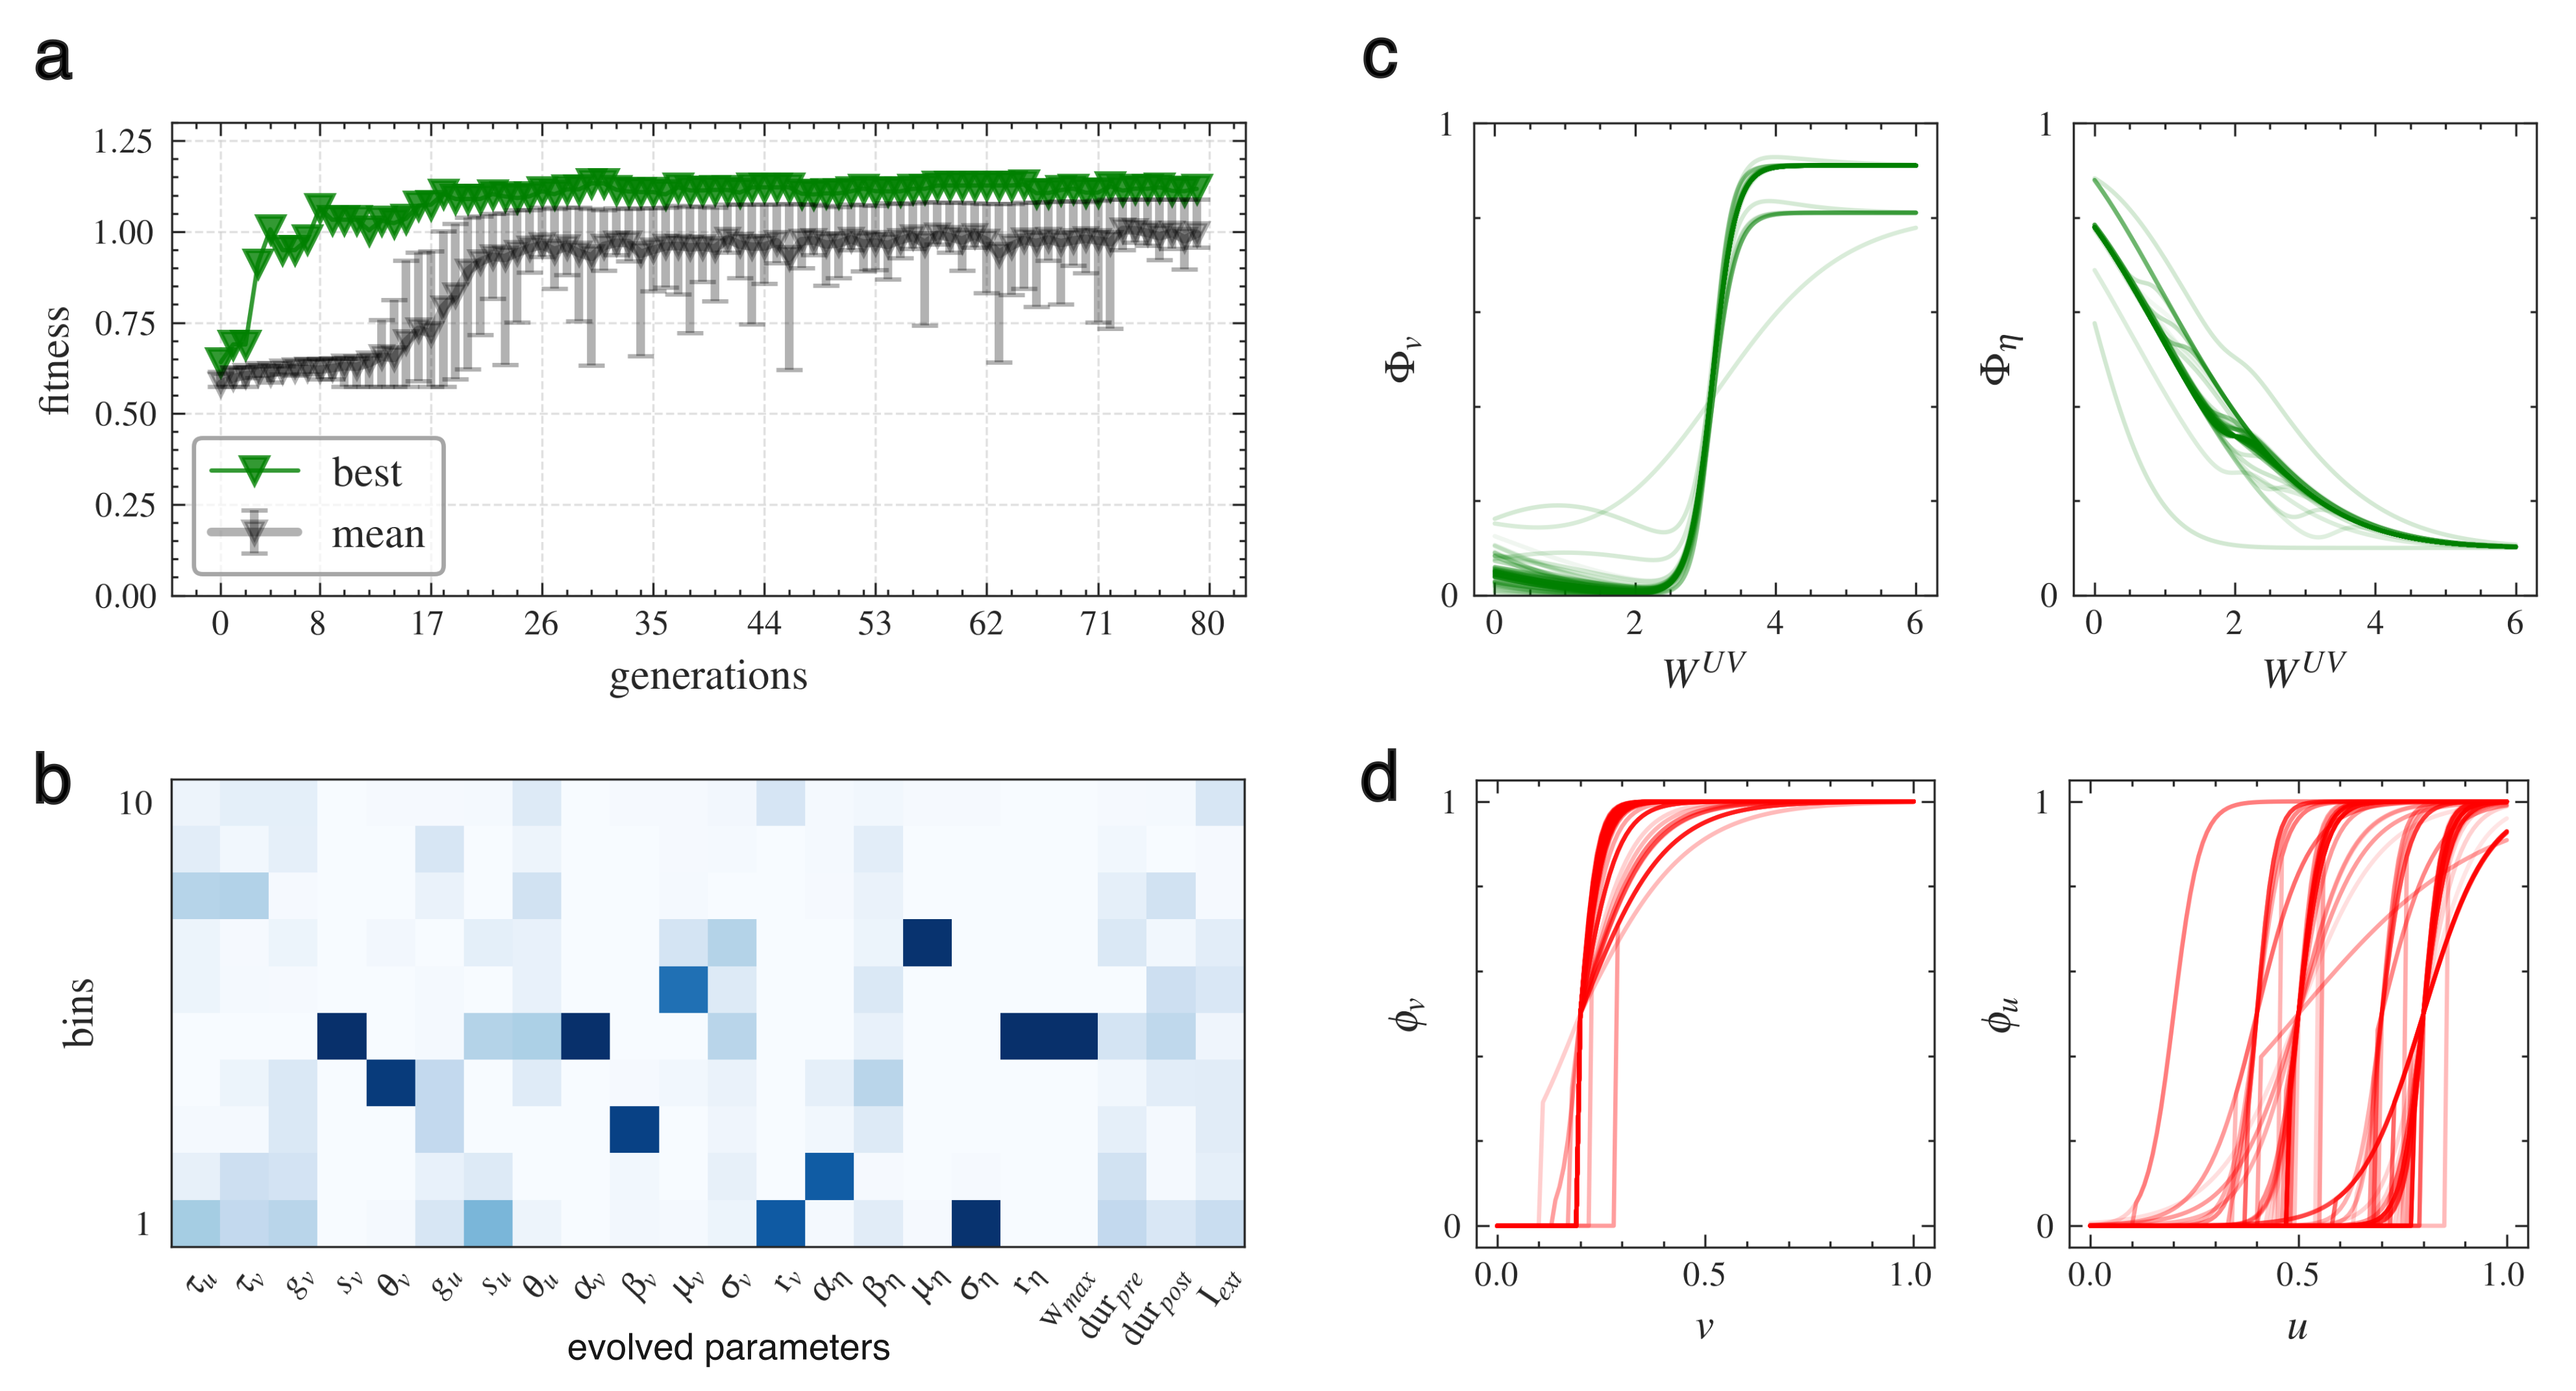
\includegraphics[width=1.0\textwidth]{figures/evolution_comp_1.png}
    \caption{\textsc{Evolution results} - \textbf{a}: \textit{top fitness, mean and standard deviation (as 16-84 percentile) of the population over generations.} - \textbf{b}: \textit{heatmap of the evolved parameters (rows) as histogram bins (y-axis) calculated from the 50 percentile of the
    population of the last generation; higher density is in dark blue} - \textbf{c-d}: \textit{Gaussian-sigmoid [c] and neural response functions [d] of the top-half of the population, the color intensity is proportional to the fitness.}}
    \label{fig:evolution}
\end{figure}

% comment on the evolved functions
\noindent The evolution progress, plot \textbf{\ref{fig:evolution}a}, showed a steady improvement over the generations, with the fitness hitting a plateau once the total reward could not get any closer to the optimum $\approx 1$ due to randomness and the finite horizon.

The evolved parameters (genome) are displayed as a frequency heatmap in \textbf{\ref{fig:evolution}b}, which was obtained from the individuals whose fitness was equal or above the median. The most relevant parameters resulted to be those concerning directly neuronal activity and learning.

More in details, the two Gaussian-sigmoid functions $\Phi_{v}, \Phi_{\eta}$, which are respectively the option value and learning rate functions, are shown in \textbf{\ref{fig:evolution}c}.
On the one hand, the learning rate function $\Phi_{\eta}$ is characterized by a decreasing curve, associated with the dominance of the right-side of the Gaussian, and a completely ignored sigmoid component.
A possible interpretation for this shape is to ensure a high learning speed when the value options are more uncertain (weak weights), and low otherwise; thus preventing overshooting and oscillations in the weight updates.
This adaptive behaviour is in line with known neuronal dynamics such as homeostatic plasticity, which works towards a stabilization of synapses, for instance through synaptic scaling and proportional updates \cite{citriSynapticPlasticityMultiple2008}.
A variable learning rate is an important feature of several plasticity rules, from the more biologically plausible like the Oja rule \cite{ojaOjaLearningRule2008} to deep learning optimizers like Adam \cite{kingmaAdamMethodStochastic2017}.

On the other hand, the option value function $\Phi_{v}$ follows instead a steep sigmoid curve.
This is consistent with the idea that the input of population $U$ to population $V$ is weighted maximally for high option values (strong synapses), whereas for weaker estimates the contributions are low or close to zero, allowing for more exploration.
Interestingly, a common feature seemed to be a slight concavity after zero, a slim influence of the Gaussian component, which might be interpreted as a sort of test for newly formed synapses. However, the size of this effect is not large.

The neural response functions are shown in \textbf{\ref{fig:evolution}d}. Both population evolved to have a similar shape, a sharp sigmoid with a clear threshold, with population \textit{U} having a more variable distribution.
The form is characterized by not allowing for a fine-grained linear reponse but rather an high-pass filter, with activity occurring only after strong excitation.
This firing behaviour is reminiscent of coincidence detector neurons, which are sometimes referred to as class III neurons with respect to their f-I curve \cite{ratteImpactNeuronalProperties2013}.


% Results: scores and brief discussion
\subsection{Environment variants and number of arms}

The model has been tested and compared with the other algorithms: Thompson Sampling (TS), $\epsilon$-Greedy, and UCB. The benchmark were the four different variants of the K-armed bandit problem listed above \ref{sec:envs}, with a variable number of arms ranging from 5 to 1000.
The results are reported in table \ref{tab:results}.
Overall, our model displayed a solid performance over all environments, most of the time being equally good or better than the other algorithms.
Interestingly, a large numbers of arms ($K$) did not present a significant challenge, as the model effectively adapted to the different environments and reward distributions.
However, this is in part due to the randomness in the assignment of arm probabilities, and the statistics of the quantity of high-reward arms as their number increases. Nonetheless, given the non-stationarity it is still a non trivial task to re-calibrate to new distributions.


% % --- table mabp
\begin{table}[ht]
\centering
\begin{tabular}{l c c c c c c c}
\toprule
\textbf{K} & \textbf{$5$} & \textbf{$10$} & \textbf{$50$} & \textbf{$100$} & \textbf{$200$} & \textbf{$1000$}\\
\midrule
TS & $0.03(8)$ & $0.02(6)$ & $0.02(7)$ & $0.04(5)$ & $0.02(3)$ & $0.16(2)$ \\
$\epsilon$-Greedy & $0.05(14)$ & $0.07(5)$ & $0.08(7)$ & $0.15(6)$ & $0.08(2)$ & $0.10(4)$ \\
UCB & $0.05(15)$ & $0.05(8)$ & $0.19(6)$ & $0.33(3)$ & $0.39(2)$ & $0.54(3)$ \\
\textbf{Model} & $\mathbf{0.08(13)}$ & $\mathbf{0.07(11)}$ & $\mathbf{0.07(14)}$ & $\mathbf{0.07(8)}$ & $\mathbf{0.09(9)}$ & $\mathbf{0.07(8)}$ \\

\midrule
TS & $0.03(6)$ & $0.08(13)$ & $0.16(6)$ & $0.19(3)$ & $0.28(7)$ & $0.34(3)$ \\
$\epsilon$-Greedy & $0.04(7)$ & $0.14(13)$ & $0.22(5)$ & $0.19(8)$ & $0.26(7)$ & $0.16(4)$ \\
UCB & $0.05(6)$ & $0.09(13)$ & $0.21(3)$ & $0.36(4)$ & $0.40(3)$ & $0.49(2)$ \\
\textbf{Model} & $\mathbf{0.13(10)}$ & $\mathbf{0.15(16)}$ & $\mathbf{0.05(6)}$ & $\mathbf{0.21(5)}$ & $\mathbf{0.26(7)}$ & $\mathbf{0.12(7)}$ \\

\midrule
TS & $0.21(22)$ & $0.22(16)$ & $0.07(5)$ & $0.10(5)$ & $0.06(4)$ & $0.21(5)$ \\
$\epsilon$-Greedy & $0.21(21)$ & $0.18(10)$ & $0.12(5)$ & $0.12(6)$ & $0.10(4)$ & $0.10(1)$ \\
UCB & $0.03(4)$ & $0.05(3)$ & $0.17(4)$ & $0.23(1)$ & $0.33(3)$ & $0.49(3)$ \\
\textbf{Model} & $\mathbf{0.00(3)}$ & $\mathbf{0.02(4)}$ & $\mathbf{0.05(3)}$ & $\mathbf{0.06(4)}$ & $\mathbf{0.08(1)}$ & $\mathbf{0.05(4)}$ \\

\midrule
TS & $0.19(21)$ & $0.43(19)$ & $0.17(10)$ & $0.11(6)$ & $0.09(6)$ & $0.19(6)$ \\
$\epsilon$-Greedy & $0.24(26)$ & $0.43(10)$ & $0.24(10)$ & $0.14(5)$ & $0.15(6)$ & $0.14(2)$ \\
UCB & $0.00(6)$ & $0.26(17)$ & $0.18(6)$ & $0.29(3)$ & $0.34(1)$ & $0.52(3)$ \\
\textbf{Model} & $\mathbf{0.00(9)}$ & $\mathbf{0.23(17)}$ & $\mathbf{0.14(7)}$ & $\mathbf{0.08(8)}$ & $\mathbf{0.06(4)}$ & $\mathbf{0.09(7)}$ \\
\bottomrule
\end{tabular}
\hfill \break
\caption{\textsc{Table of performance} - \textit{From the top: results for MAB-P, MAB-D, MAB-$\sin$, MAB-$\sin$P for different numbers $K$ of arms. Average regret and standard deviation (2 decimal places) over 2 trials of 2000 rounds each averaged over 5 simulations.}}
\end{table}\label{tab:results}



% How the models work and compare
\subsection{Analysis of dynamics and robustness}

% entropy over rounds
\subsubsection{Entropy analysis}\label{sec:entropy}
\noindent For a better understanding of the qualitative differences between the models, we analyzed the progress over the rounds by tracking the selected arms in a simple piecewise stationary distribution environment.
The simulation was run for $3$ trials with $2000$, and averaged over $5$ iterations.
Additionally, in order to quantify the variability of the decision policy at a given time and highlight the particularity of each decision-making behaviour, we calculated the entropy of the probability distribution $p$ of chosen arms, calculated over a window of 20 rounds, as $H=-\sum^{K}_{i} p_{i}\log(p_{i})$.
The unit of entropy is in nats, and it ranges from $0$ (no uncertainty) to $\log_{e}(K)$ (maximum uncertainty).
In figure \ref{fig:entropy_fig1}-\textbf{a}, it is plotted for each model the raster plot of selected arms together with its level of entropy. The reward probability distribution over the arms has an average of $H=2.02$.

As expected, the shape of the entropy curve expresses the inherent strategy adopted by each model.
In particular, the UCB algorithm showed the highest variability, marked by a persistent exploratory behaviour throughout the trials despite converging to reward options. Thompson Sampling was able to reach most solutions, although with difficulty in adapting to new reward distributions
leading to high entropy levels.
$\epsilon-$Greedy also showed a good performance quite reliably, with the greedy strategy assuring low entropy for most of the rounds.
Similar behaviour was observed for our model, which was able to reach the optimal policy and maintain it over time, with entropy peaking mostly at the beginning of the trials and being, on average, the lowest among all models.
Indeed, the dynamics of our model make it particularly suited for the task of non-stationary K-armed bandits, as it is able to quickly adapt to new reward distributions and firmly maintain a greedy policy.

\begin{figure}[H]
    \centering
    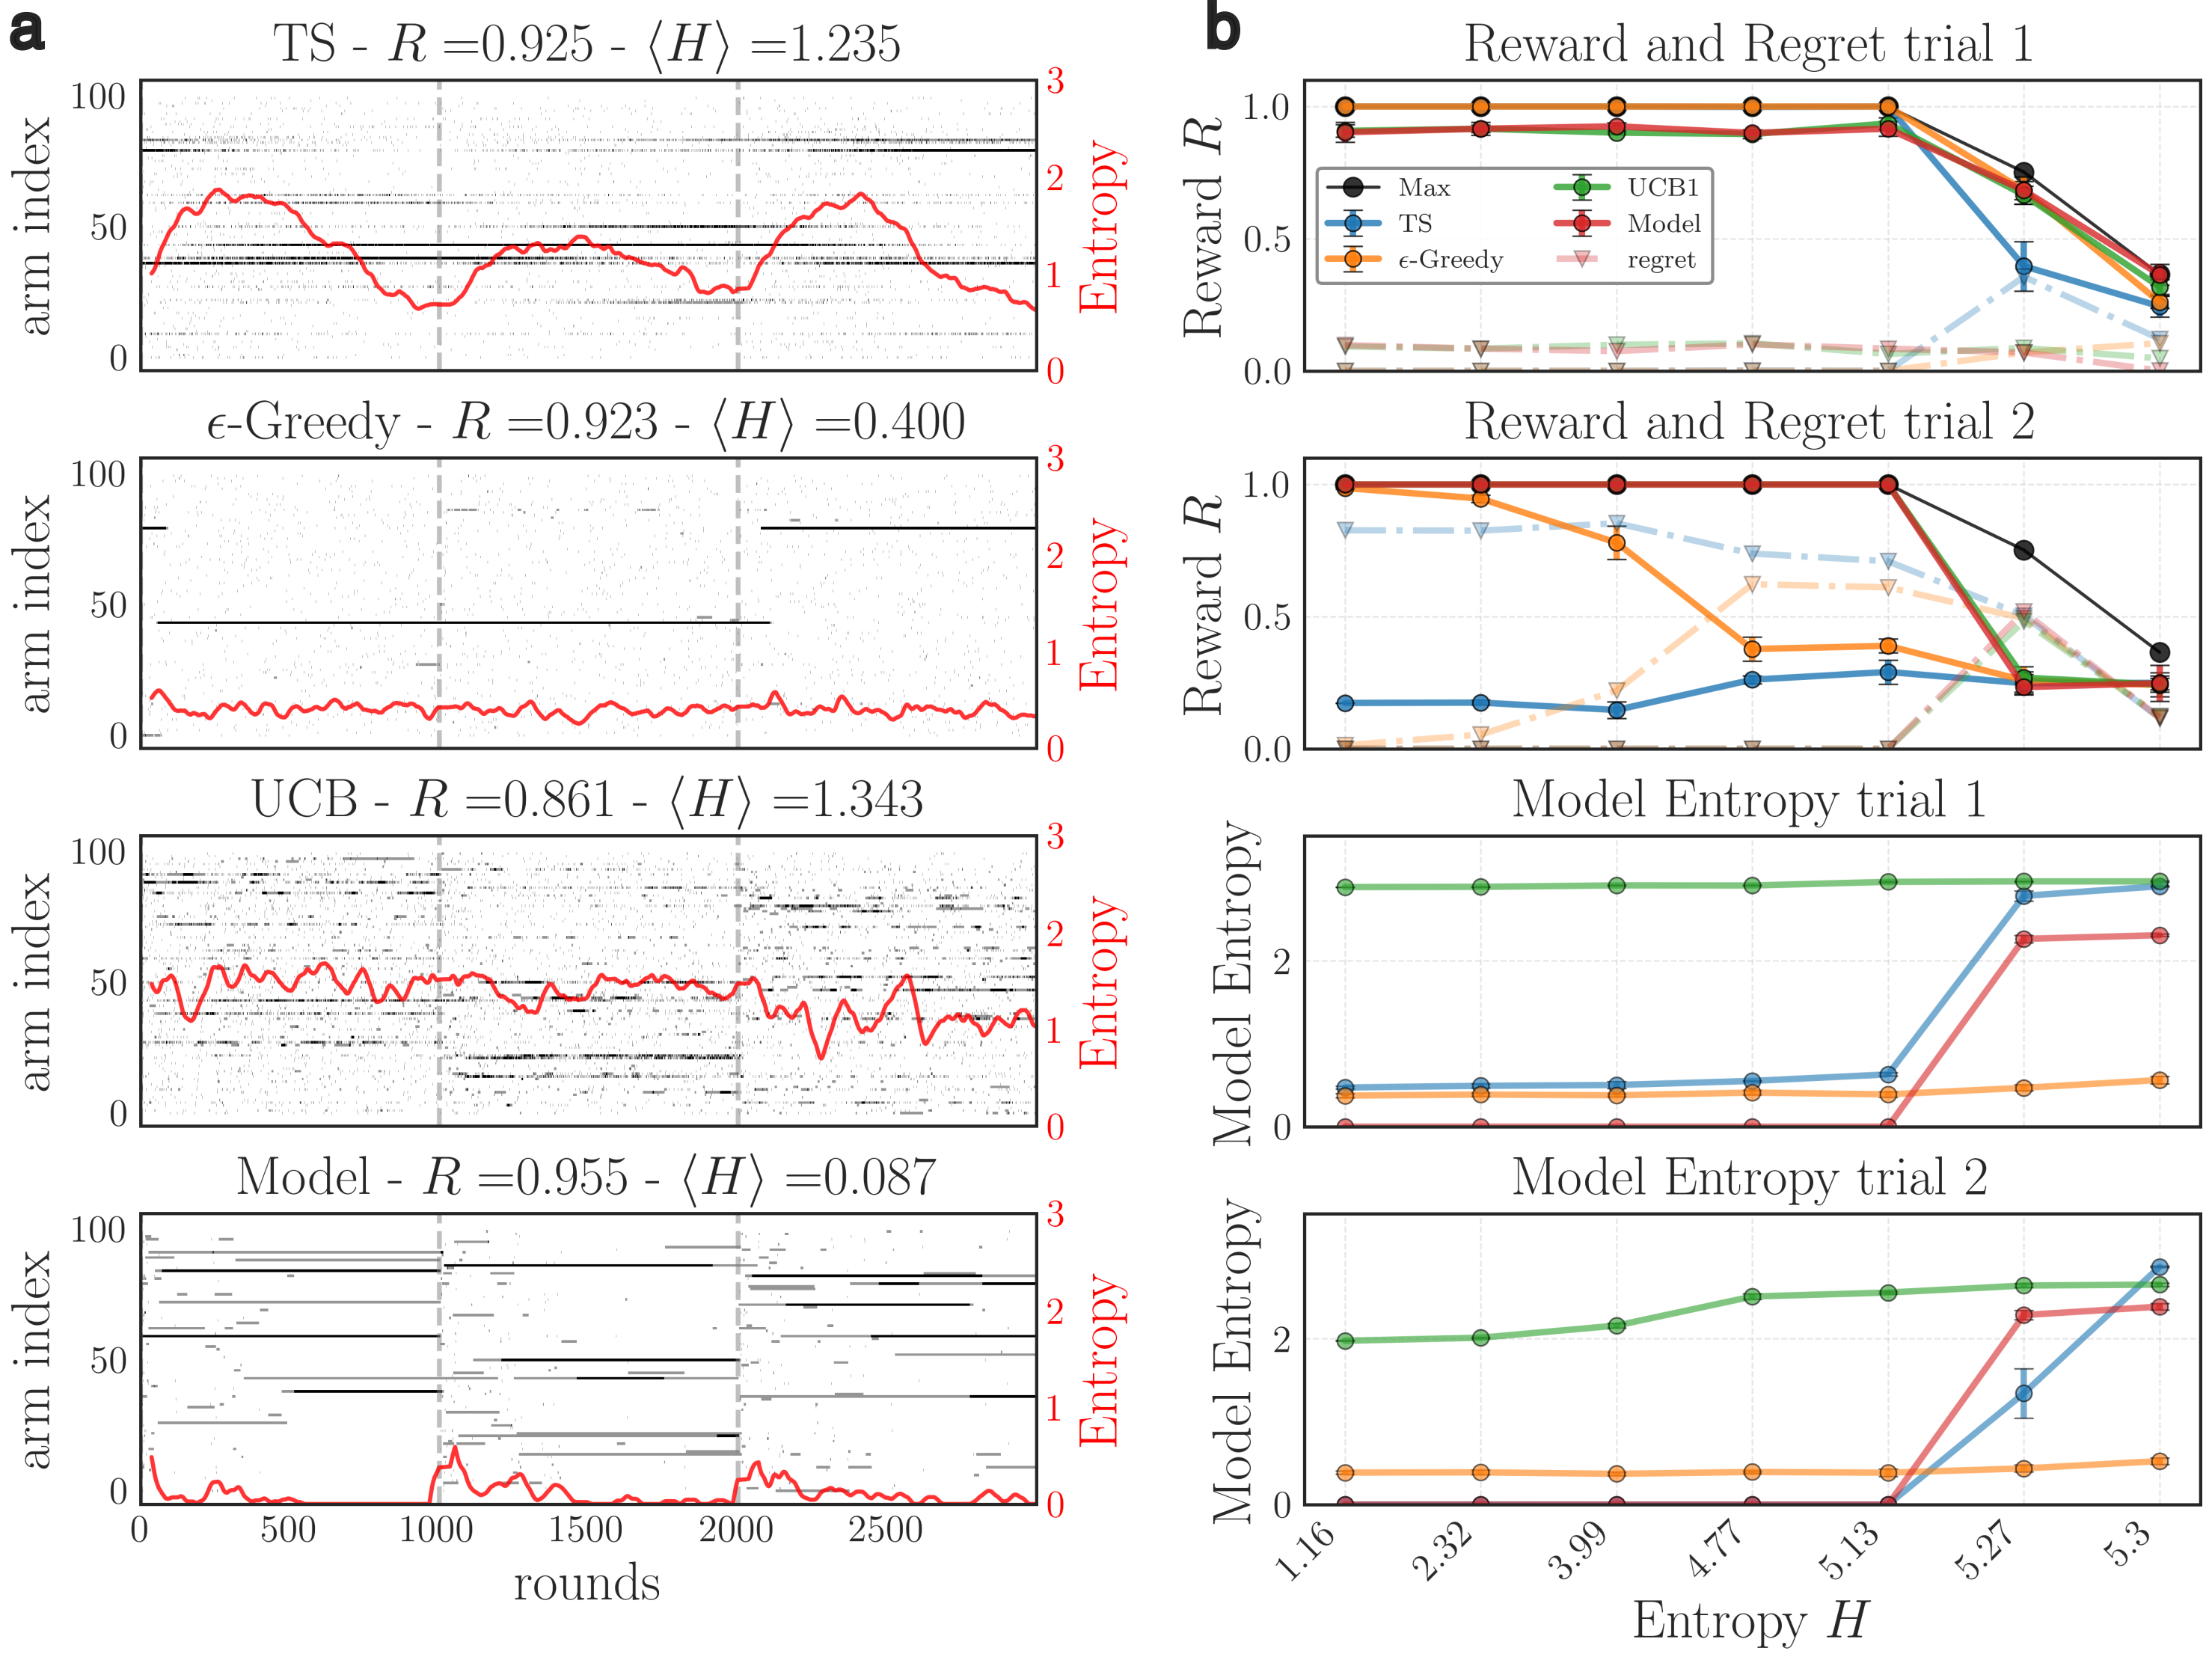
\includegraphics[width=1.0\textwidth]{figures/entropy_main_plot_2.png}
    \caption{\textsc{Decision-making dynamics for different models} - \textbf{a}: \textit{Each plot display the results from one model. The raster plots (black dots) show the arms selected at each round.
The red lines represent the entropy level, calculated from the distribution of selections over the preceeding 20 rounds, smoothed with a 30-steps moving average. In the plot titles, the total reward and average entropy over all trials are also reported.}
 - \textbf{b}: \textit{the top two rows display  the average reward for trial 1 and 2 obtained by each model for increasing levels of entropy (in nats) in the reward distribution; a dashed line is the regret with respect to the upper bound (black solid line). The two bottom average entropy of the selections for the first and second trial of the simulation, each with 2000 rounds. -
\textbf{c}: \textit{testing of the model to a 500 arms MAB-P enviroment for three epochs. - \textbf{d}: representation of the arms reward distributions for different levels of entropy, aligned with the x-axis in plot \textbf{b}.}}}
    \label{fig:entropy_fig1}
\end{figure}


% how robust and structure is the model
% \subsubsection{Robustness}

% robustness
\noindent Then, we sought to investigate the robustness of the model, quantified as the capacity to endure increasing levels of entropy in the reward distribution.
The simulation was done in a piecewise stationary environment with $K=200$ in two trials averaged over 5 independent runs, and it is showed in figure \textbf{\ref{fig:entropy_fig1}b}.
The distributions were chosen such to have only one strongly rewarding arm, in order to highlight the models ability to find it.
In plot \textbf{\ref{fig:entropy_fig1}d}, an example of distributions is plotted in \textbf{\ref{fig:entropy_fig1}d} and are aligned with the x-axis in plot \textbf{\ref{fig:entropy_fig1}b}.
For more details about the distribution see the appendix \ref{sec:appendix_entropy}.
In the top two plots, it is shown the average reward and regret obtained by each model against the reward distribution entropy for the two trials.
The results reported how all models are capable of robust performance in the first trial even in the presence of high uncertainty.
In the second trial, $\epsilon$-Greedy and Thompson Sampling suffered the increasing difficulty of switching arms, probably due to their conservative approaches. However, this challenge afflicted UCB and our model only with higher entropy levels, recognizing their adaptability.

Another perspective to this analysis was given by the two bottom plots, which showed the average entropy over the trials.
Overall, there was the unsuprising trend of increasing selection entropy with the entropy of the reward distribution. Nonetheless, striking is the exception of Epsilon-Greedy, which still maintained a constant level throughout.
UCB displayed the highest average values, while Thompson Sampling followed with some delay.
On the other hand, our model display a more abrupt change, going from a state of very low to high variability, sign of a solid exploratory behaviour.



